\documentclass[letterpaper]{article}
\usepackage{graphicx}
\usepackage[left=3cm,top=2cm,bottom=2cm,right=3cm]{geometry}
\usepackage[title,titletoc]{appendix}
\usepackage{authblk}
\usepackage[parfill]{parskip}

\title{An FPGA-based Pattern Recognition Associative Memory
\\Fermilab Technical Memo TM-XXXX-X}

\author[1]{Jamieson Olsen}
\author[1]{Tiehui Ted Liu}
\author[1]{Jim Hoff}
\author[1]{Jin-Yuan Wu}
\author[1,2]{Zijun Xu}

\affil[1]{Fermi National Accelerator Laboratory\footnote{Operated by Fermi Research Alliance, LLC under Contract No. DE-AC02-07CH11359 with the United States Department of Energy.}, Batavia, Illinois USA}
\affil[2]{Peking University, Peking CHINA}

\date{\today}


\renewcommand{\topfraction}{0.9}	% max fraction of floats at top
\renewcommand{\bottomfraction}{0.8}	% max fraction of floats at bottom
%   Parameters for TEXT pages (not float pages):
\setcounter{topnumber}{2}
\setcounter{bottomnumber}{2}
\setcounter{totalnumber}{4}     % 2 may work better
\setcounter{dbltopnumber}{2}    % for 2-column pages
\renewcommand{\dbltopfraction}{0.9}	% fit big float above 2-col. text
\renewcommand{\textfraction}{0.07}	% allow minimal text w. figs
%   Parameters for FLOAT pages (not text pages):
\renewcommand{\floatpagefraction}{0.7}	% require fuller float pages
% N.B.: floatpagefraction MUST be less than topfraction !!
\renewcommand{\dblfloatpagefraction}{0.7}	% require fuller float pages
% remember to use [htp] or [htpb] for placement

% \setlength\parindent{0pt}

\begin{document}

\maketitle

\begin{abstract}
\noindent Pattern recognition associative memory (PRAM) devices are parallel processing engines which are used to tackle the complex combinatorics of track finding algorithms, particularly for silicon based tracking triggers. PRAM development has been mostly limited to the realm of ASICs, which often leads to lengthy and expensive design cycles. FPGAs allow for quick iterations, making them an ideal hardware platform for designing and evaluating new PRAM features before committing to silicon. In this paper we present our FPGA-based PRAM designs and discuss how logic blocks which were originally developed for ASICs have been redesigned to take advantage of modern FPGA architectures.
\end{abstract}

\newpage
\tableofcontents
\listoffigures
\listoftables

\newpage

\section{Introduction}

Pattern recognition associative memory (PRAM) devices are massively parallel processing engines which can be used to tackle the complex combinatorics of track finding algorithms, particularly for silicon based tracking triggers at high luminosity LHC. Until recently PRAM development has been limited mostly to the realm of ASICs, often a lengthy and expensive process. FPGAs however allow for quick iterations and low cost design cycles, making them an ideal hardware platform for 
designing and evaluating new PRAM features before committing them to silicon. 

It is in the implementation details, however, that the differences between the ASIC and FPGA PRAM designs become apparent. In our experience we have found that logic blocks which have been optimized for fine-grain ASIC architectures do not implement efficiently in coarse-grain FPGA logic cells without significant redesign. For example, the CAM cell is fully programmable and requires registers to store the pattern bits. These registers can be implemented in an ASIC with just a few transistors, but in an FPGA these register bits consume entire flip flops and this leads to an inefficient use of logic resources. Our solution to this challenge was to completely redesign the CAM cell to take advantage of the modern FPGA logic cell features.

\section{PRAM Overview}

\subsection{RAM and CAM Architectures}

To understand how a PRAM device works, we first begin with a brief description of a Random Access Memory (RAM) and Content Addressable Memory (CAM). In a conventional RAM device the user inputs an address and the RAM outputs the data value stored at that address. In contrast, CAM can be thought of as an inverse RAM: the user presents a data value and the CAM device outputs the address (or addresses) of the memory location which contains that data. Internally RAM and CAM devices are \emph{very} different. RAM is typically constructed from storage elements followed by a large, wide multiplexer driven by the input address bus. In a CAM device the input data bus is distributed to all storage elements which then perform comparisons in parallel. Thus each storage element in the CAM contains match logic followed by wide priority decoder used for address generation. If the CAM device supports reading out more than one address the complexity of the backend priority decoder logic grows substantially.

\subsection{PRAM Architecture}

PRAM builds upon the high performance parallel search nature of CAM and in a sense can be thought of as a ``CAM of CAMs". Rather than match on a single data value, PRAMs support multiple data values, input on separate buses which we refer to as layers.A PRAM device is constructed from an array of PRAM cells followed by backend serialization logic as shown in Figure \ref{pramblock}.

\begin{figure}
\centering
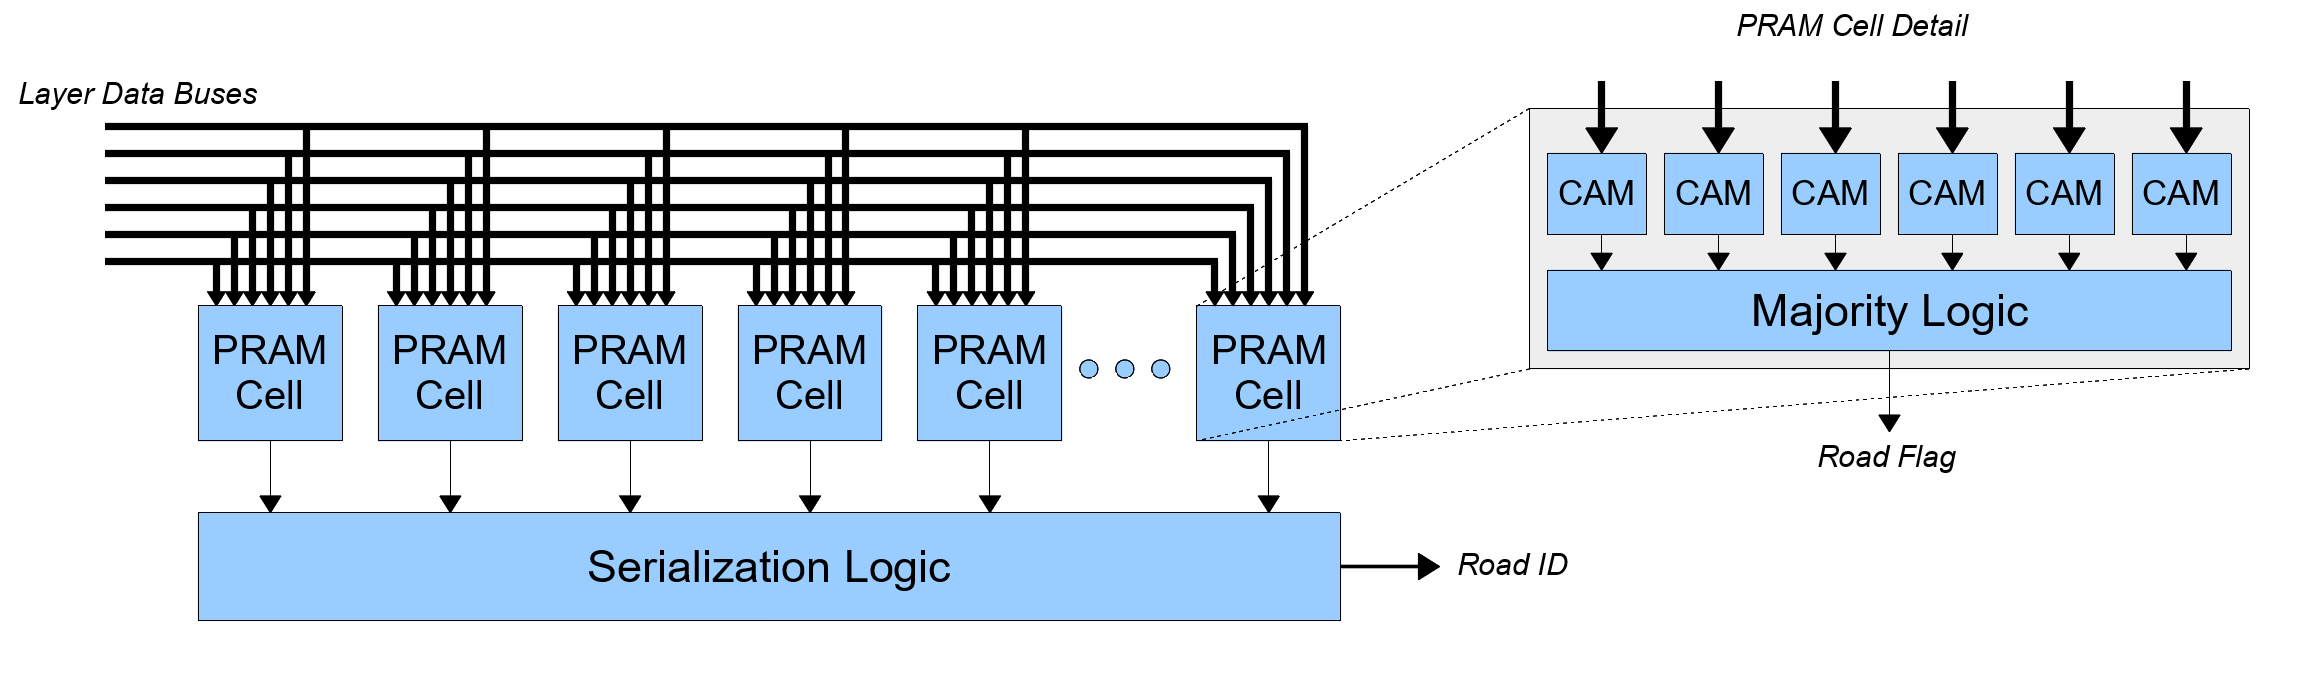
\includegraphics[width=14cm]{pram.png}
\caption[PRAM Block Diagram]{PRAM block diagram with PRAM cell detail shown on the right.}
\label{pramblock}
\end{figure}

\subsubsection{PRAM Cell}

If our reference designs the PRAM Cell consists of 6 small CAMs followed by a majority logic block. Each CAM is 10 bits wide and only one word deep. In other words, this CAM is simply a register in which the user can store a 10 bit pattern. When the input data bus matches the stored pattern the CAM output bit goes high. Depending on the implementation details the CAMs may also support ternary ('X') bits in the pattern.

The outputs from the six CAMs in the PRAM cell then feed into a configurable majority logic block. Here we can choose how tight or loose the match logic will be. A perfect match means that all 6 CAMs must report a match in order to set the output Road Flag. A loose match may mean that 5 out 6 CAMs match. Typically the majority logic configuration is set globally, affecting all PRAM Cells in the device. Once the Road Flag output goes high it latches and remains high until it is reset by the End of Event (EOE) control signal.

\subsubsection{Serialization Logic}

The backend serialization logic sees the array of Road Flags and outputs the index (called a Road-ID) of any set Road Flag(s). Essentially this logic block consists of a large, wide priority encoder with logic added to implement sequential readout of multiple set Road Flags. The serialization logic represents perhaps the most significant difference between the ASIC and FPGA PRAM implementations. ASIC designers are able to leverage specialized asynchronous sorting structures (i.e. Fischer Trees) to build the priority encoder logic. While it is possible to build Fischer Trees in the FPGA fabric, the wide and deep asynchronous logic functions result in massive LUT usage and unacceptably slow performance. The FPGA designs must utilize different structures to efficiently build priority encoders with thousands (even tens of thousands) of input bits.

\subsubsection{Pipelined Operation}

PRAM throughput can be increased by separating the CAM functions and backend serialization functions, allowing for concurrent read-in and read-out operation. The Road Flag registers are a natural choice for a pipeline stage boundary: the first stage consists of PRAM cells which process data for the current event; and in the second stage the backend serialization logic processes the Road Flags from the previous event. The EOE control signal is used to reset all PRAM cells and at the same time copy the Road Flags into registers in the backend serialization block.

\section{FPGA Implementation}

\subsection{I/O Interface}

FPGA I/O resources are flexible and highly configurable; high speed serial (MGT) as well as wide parallel buses are supported. This allows for many different system interface options to be evaluated in our FPGA PRAM design. The current FPGA PRAM interface is modeled after our latest PRAM ASIC design and consists of wide parallel single-ended buses. DDR transmission is used to clock data into the PRAM on rising and falling edges of the master clock which is nominally 240MHz LVDS.

The PRAM input bus is 64 bits wide and organized as 6 layers of 10 bits each plus 4 control bits. A Valid bit is not used on the 6 individual layer data buses; therefore the value 0000000000 is reserved to indicate no data and care must be taken that no CAM cells should match on this pattern. The control bits are used to encode the EOE marker and various other commands such as downloading patterns to the CAM cells and setting the majority logic MODE bits. One control bit is used for a parity check over the entire 64 input word. Since the PRAM input is DDR it requires only 32 single-ended I/O pins on the FPGA. The 64 bit bus used here is advantageous because it allows for a natural transition from wide parallel input buses to a high speed serial MGT receiver (natively 64 bits) in future designs.

The PRAM output interface is also single-ended DDR and is used for sending a valid bit along with the Road-ID field. We reserve 18 bits for the Road-ID field, allowing for a single PRAM device to support up to 256k patterns. A phase-aligned copy of the master clock is also provided on the PRAM output interface. Future PRAM designs may replace the parallel output bus with an MGT high speed serial transmitter.

\subsection{PRAM Cell}

The PRAM cell consists of 6 small CAMs plus majority logic. Significant effort has gone into designing the PRAM cells to be as compact as possible given the building blocks available in the FPGA logic cells.

\subsubsection{CAM Design}

\begin{figure}
\centering
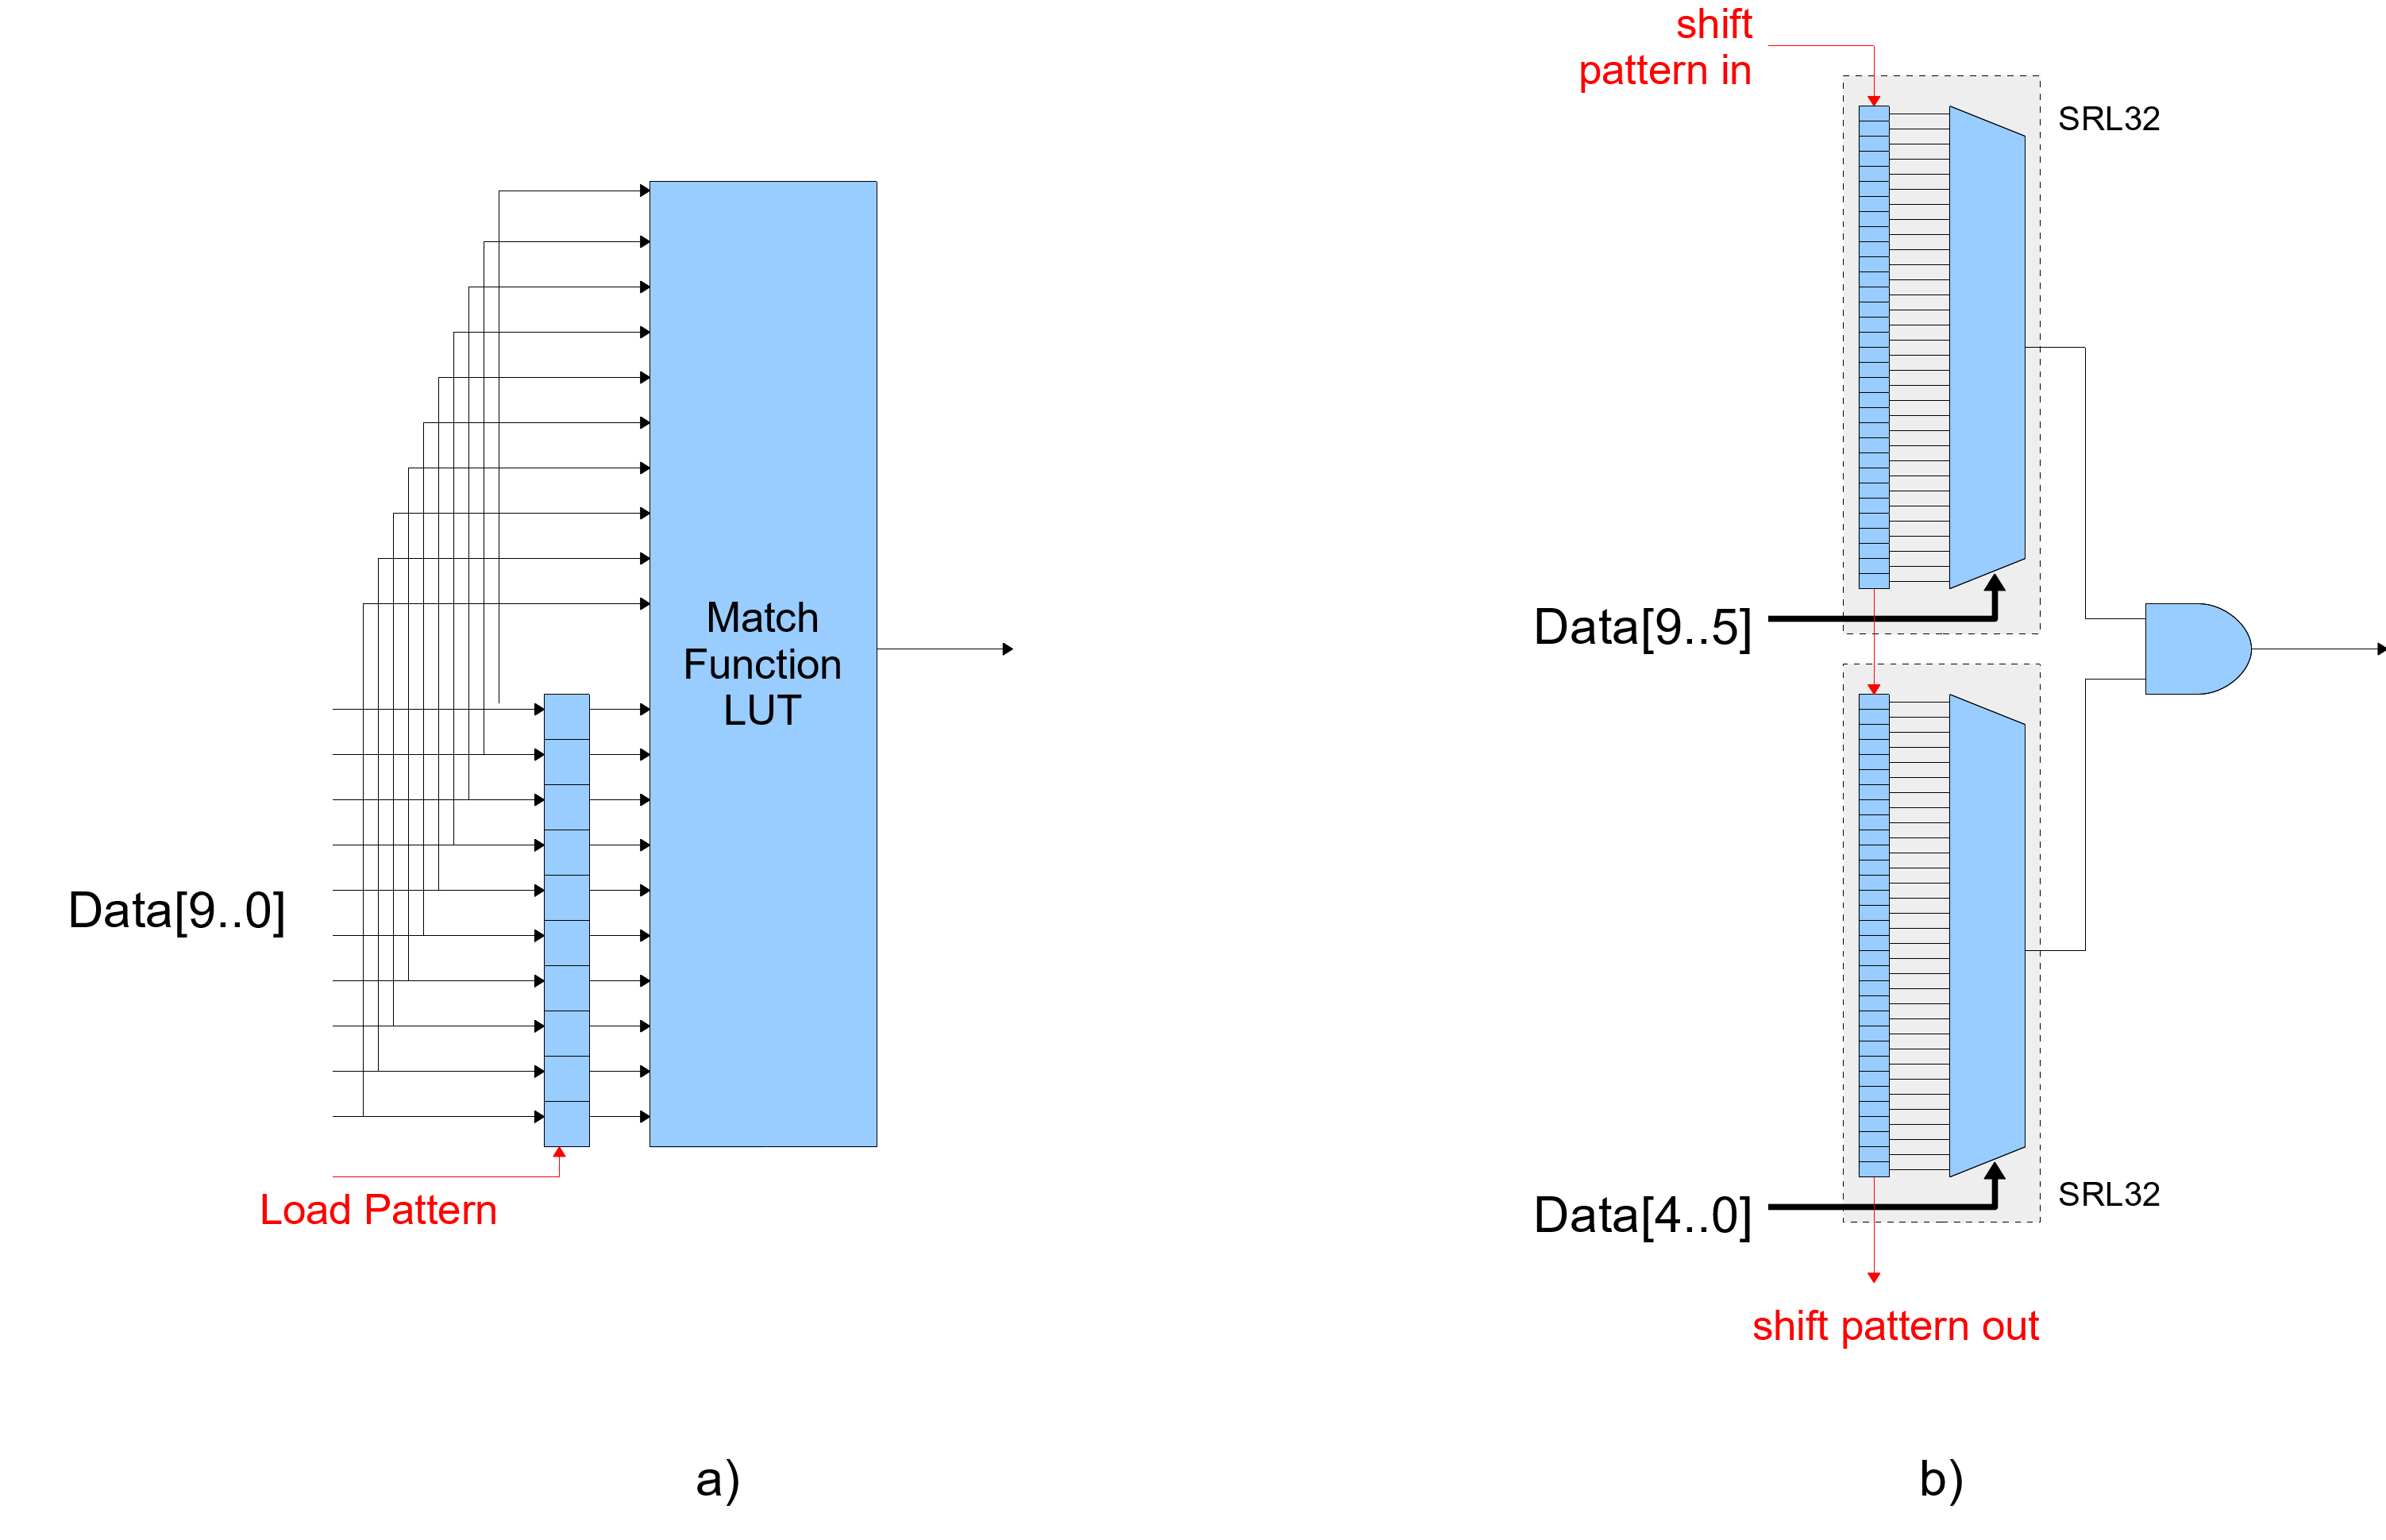
\includegraphics[width=14cm]{cam.png}
\caption[Two CAM Designs]{Comparison of two 10 bit CAM designs. The CAM on the left supports parallel loading of a 10 bit pattern and is based on the PRAM ASIC design. The CAM on the right has been redesigned to take advantage of the 32-bit shift register primatives available in UltraScale FPGAs.}
\label{camfigs}
\end{figure}

Each CAM is tiny and stores only a single user-programmable 10 bit value. In the simplest terms the CAM can be thought of as a 10 bit register followed by a 20 bit AND gate: when the layer input bus matches the contents of the register the AND gate output goes high. Early FPGA implementations of the CAM were based on a direct translation of the ASIC design. These ``classic" parallel load CAM cells utilized discrete D-Flip Flop registers and wide AND function made out of LUTs as shown in Figure \ref{camfigs}a. It was quickly determined that this simple approach resulted in unacceptably inefficient FPGA resource usage, and that the CAM needed to redesigned to better match a modern FPGA logic cell.

Figure \ref{camfigs}b shows an updated CAM design based around a pair of shift register primitives (SRL32). Originally intended to be used as a variable depth shift register, each SRL32 consists of a serial-loadable 32 bit shift register followed by a 32 bit MUX. Here the SRL32 is used to create a 5 bit CAM where the pattern is stored in the shift register bits and the data input drives MUX select lines. Essentially this CAM behaves like a 5 input LUT with one important distinction: the stored pattern can be updated by the user at run time without reconfiguring the FPGA or rebuilding firmware.

This new CAM design is \emph{significantly} smaller than the ``classic" CAM and requires only two SLICEM type logic cells in Xilinx UltraScale devices. The new CAM design has the added benefit of supporting ternary (don't care, 'X') values in any bit position of the stored pattern with no additional logic resources consumed.

\subsubsection{Majority Logic}

The Road Flag output of each PRAM cell set is set whenever the 6 CAM cells simultaneously report a match condition as defined by the majority logic block. The global MODE control bits determine how stringent the match condition is. The PRAM supports the following modes: Perfect Match (all 6 CAMs must match); Missing-1 (5 out of 6 CAMs match); and Missing-2 (4 out 6 CAMs match). Once a PRAM cell asserts the Road Flag output it remains set until the PRAM cell is reset by the End-of-Event control signal.

\subsection{Serialization Logic}

\begin{figure}
\centering
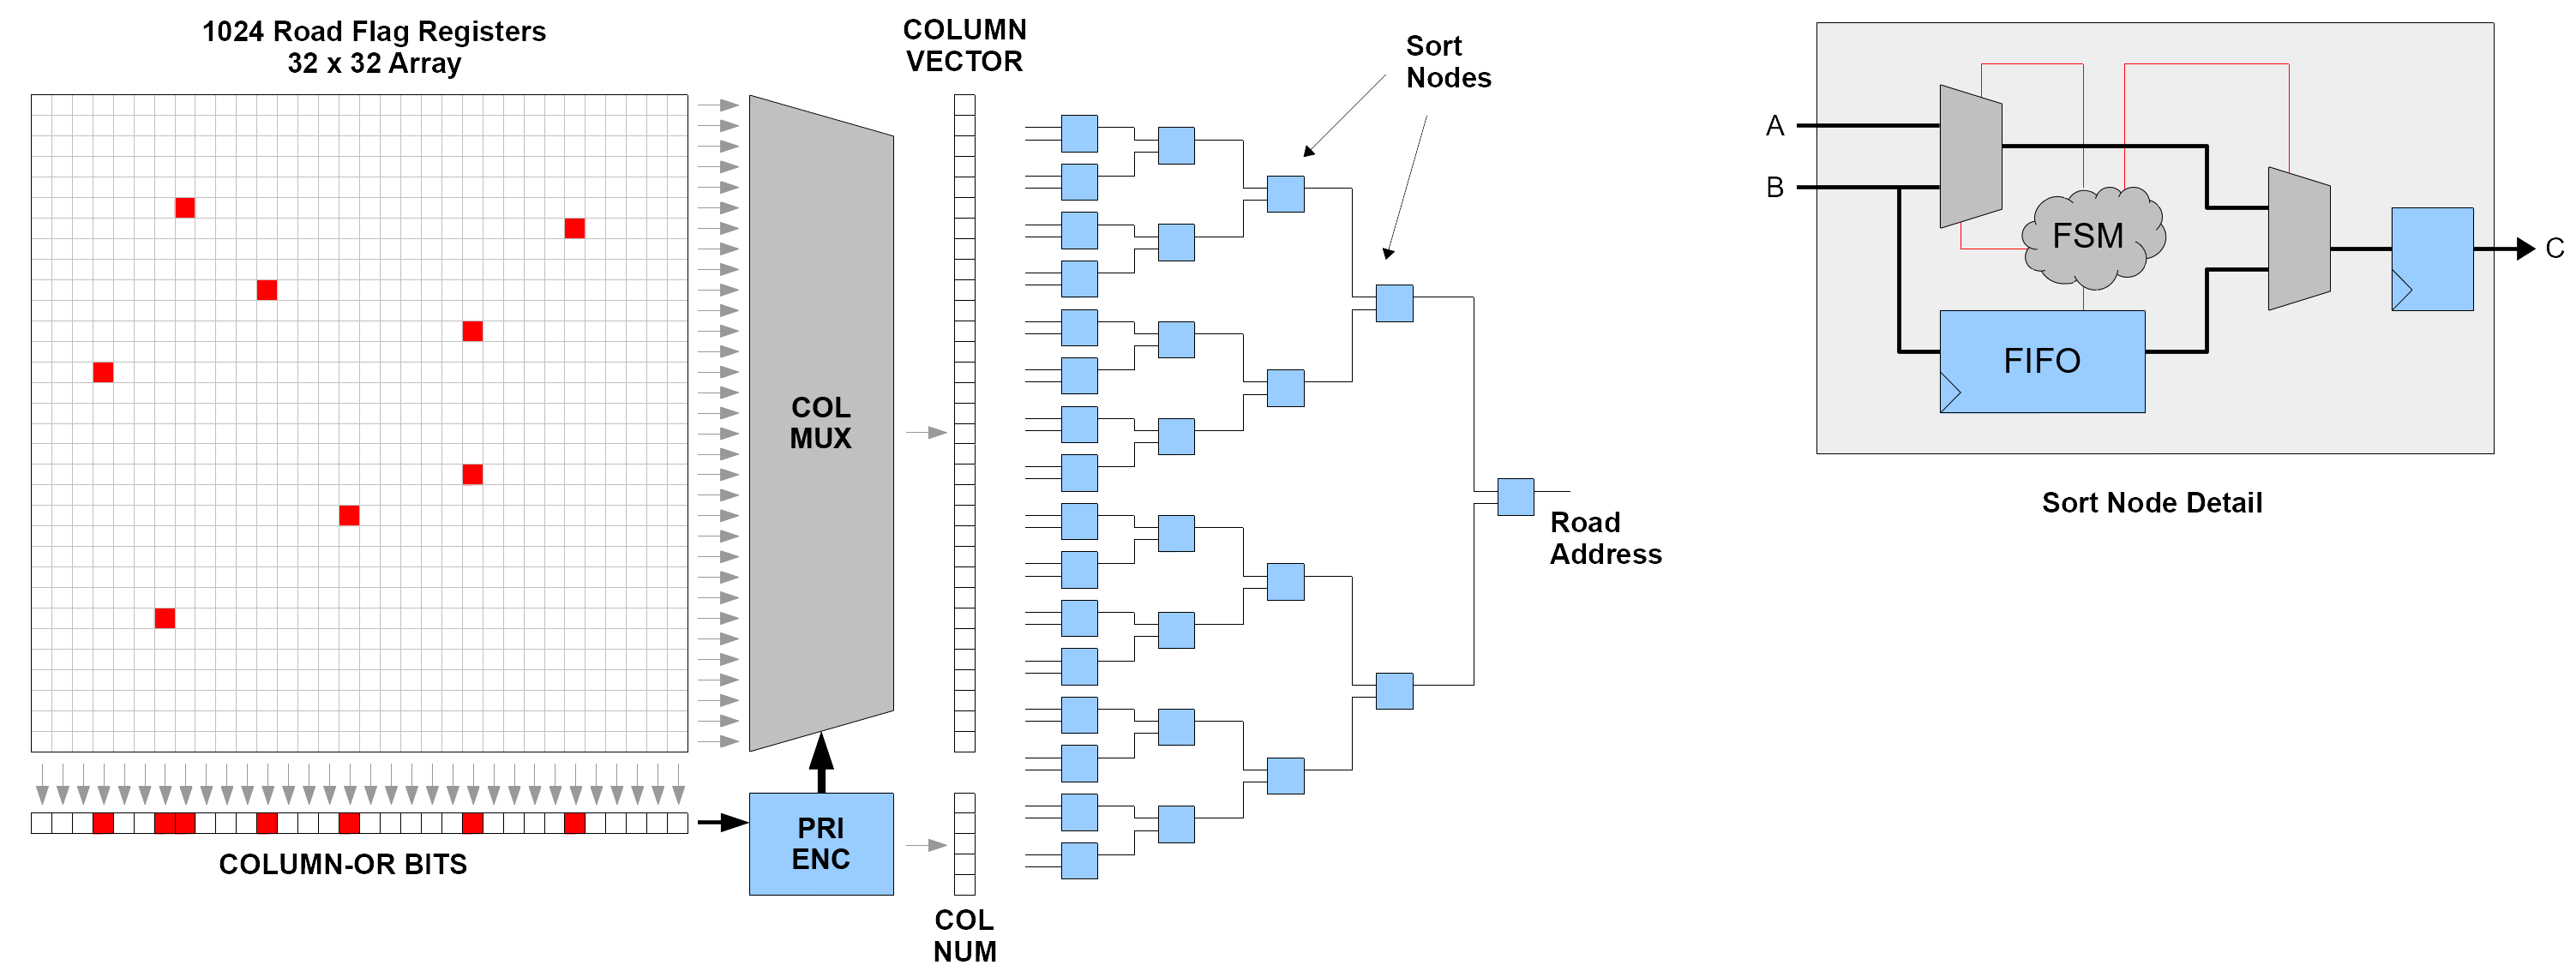
\includegraphics[width=14cm]{backend.png}
\caption[PRAM Serialization Logic]{PRAM Serialization Logic pipeline. This design supports 1024 Road Flags in a 32 x 32 matrix. Latency is 7 clock cycles. Internally buffered sort node detail is shown in the right. In this example set Road Flags are shown in red.}
\label{backend}
\end{figure}

The Serialization Logic block for a 1024 pattern PRAM design is shown in Figure \ref{backend}. This block reports the index or address of each set Road Flag bit in the PRAM. These addresses, called Road-IDs, are output sequentially, preferably in zero suppressed format. This logic block must be designed in such a way that it can gracefully scale from small PRAMs (1k patterns) to large PRAMs (100k patterns).

\subsubsection{Road Flag Registers and Selection MUX}

When the End-of-Event signal is observed the Road Flag array is loaded into registers and the serialization process begins. First, the logical OR of the Road Flags in each column are stored in registers. These column bits are used by the synchronous 32-bit ``peel away" priority encoder and MUX to quickly and sequentially select populated columns which are sent down the row serialization pipeline. 

For example, in Figure \ref{backend} there are 8 Road Flags set in columns 3, 6, 7, 11, 15, 21, and 26 (counting from left to right). On the first clock edge after End-of-Event the priority encoder determines that bit 3 is set, and the large column MUX then selects column 3 for passing along to the sort nodes. On the next clock cycle column 6 is passed along, and so on until all columns with set Road Flags have been selected.

\subsubsection{Merge Sort Logic}

The row serialization pipeline consists of 5 stages of internally buffered sort nodes, shown inset in Figure \ref{backend}. Each sort node is controlled by a finite state machine (FSM). Based on the inputs A and B and FIFO empty status the FSM determines which Road-ID is sent to output C. The FIFO, which is constructed from distributed RAM elements, is deep enough to insure that no Road-ID values are lost.

The first Road-ID value is output from the final sort node exactly 7 clock cycles after the End-of-Event control signal is asserted. All Road-IDs are reported sequentially with no gaps between (fully zero suppressed output). For PRAM designs larger than 1k patterns the 32x32 serialization block is instantiated multiple times, and the outputs are joined together with additional sort nodes to arrive at a single output bus. In such cases the output latency is increased by a few additional clock cycles.


\subsection{Device Resources and Performance}

\begin{figure}
\centering
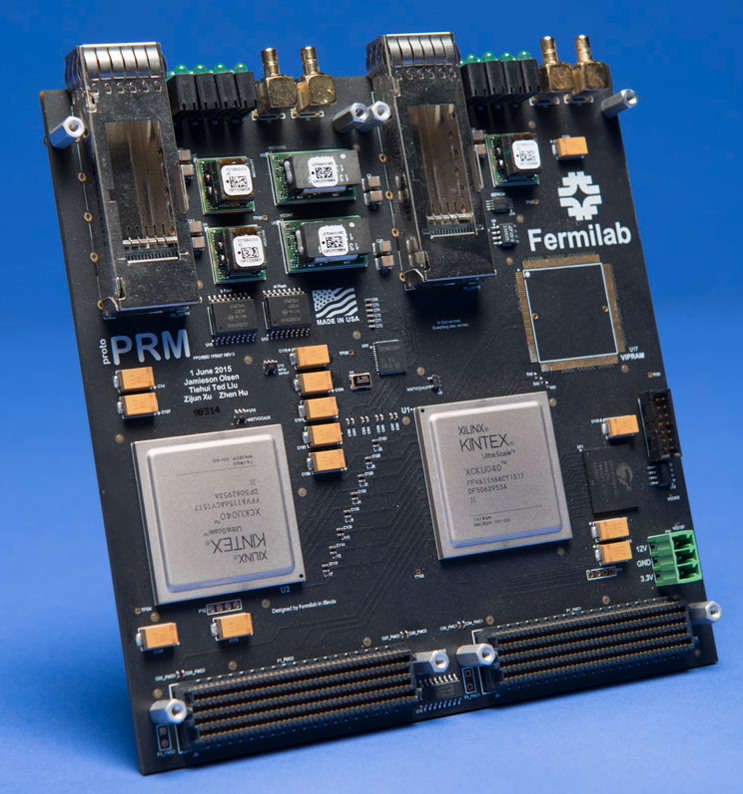
\includegraphics[width=10cm]{prm.png}
\caption[Pattern Recognition Mezzanine]{Pattern Recognition Mezzanine (PRM). This board has two Kintex UltraScale KU060 FPGAs installed. The FPGA on the right is the Master and is responsible for data organization and track fitting. The FPGA on the left is the Slave and is used to test various PRAM designs.}
\label{prm}
\end{figure}

After passing functional simulation and static timing analysis checks the PRAM FPGA designs were verified by real-world testing using the Pattern Recognition Mezzanine board shown in Figure \ref{prm}.

Various size PRAM designs have been built using the Xilinx Vivado 2017.4 tools and the target device is the Kintex UltraScale KU060 FPGA in the -2 speed grade. FPGA device resources are shown in Table \ref{TableFPGA}. In all cases the PRAM design uses 6 input buses/layers of 10 bits each, and the CAMs were constructed using two SRL32 type shift registers (which show up as LUTRAM resources). 

In all cases timing constraints were met with a clock rate of 240MHz. 

\begin{table}[htp]
\centering
\caption{PRAM FPGA Resources KU060} 
\label{TableFPGA}
\begin{tabular}{|l|l|l|l|}
\hline
PRAM Patterns & LUT & LUTRAM & FF   \\
\hline
1k & 11\%  & 14\%           & 2\%  \\
4k & 46\%  & 58\%           & 7\%  \\
8k & 90\%  & 113\% (failed) & 17\% \\
\hline
\end{tabular}
\end{table}

%\newpage
\section{Pattern Density Optimization Studies}

In this section we explore how the PRAM design would change if the run-time pattern loading feature was abandoned. Rather than load patterns into programmable CAMs now the patterns are hard-coded in the firmware. The advantage of this approach is that the size of the PRAM cell shrinks dramatically, leading to a significant increase in pattern density. A disadvantage of this approach is that with each pattern change the complete FPGA design will need to be rebuilt (synthesis and implementation requires about 1 hour typically).

\begin{figure}
\centering
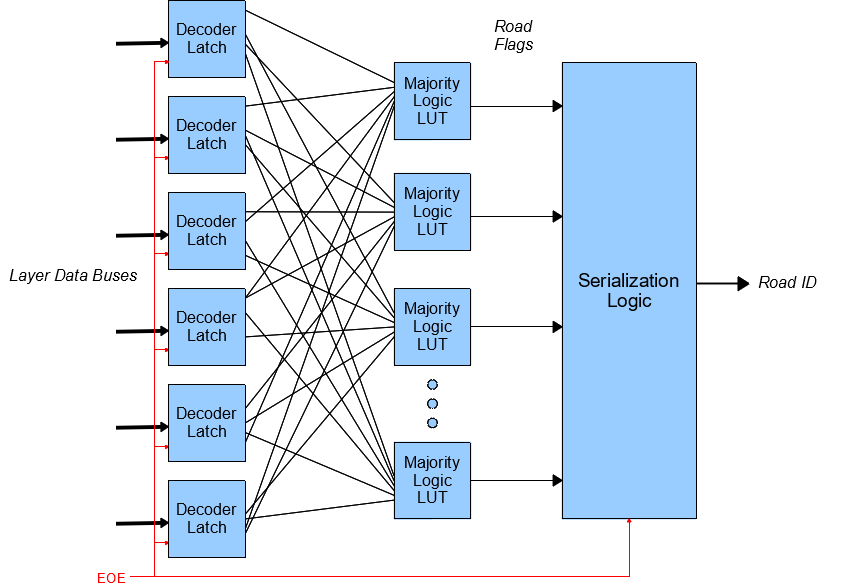
\includegraphics[width=14cm]{densepram.png}
\caption[PRAM Designed for Maximum Pattern Density]{An alternative PRAM design optimized for maximum pattern density. The pattern is defined by the interconnection between the Decoder Latch outputs and the majority logic LUTs. The programmable CAMs have been removed from the design.}
\label{densepram}
\end{figure}

One possible alternative PRAM design in shown in Figure \ref{densepram}. The front end logic has changed and now each layer input bus terminates at a 10x1024 bit decoder with latching output bits. Once set, the decoder output bits remain set until cleared by the EOE control signal. 

The programmable CAMs have been eliminated from this new design, and the resultant PRAM cell is simply a LUT which performs the majority logic function. In this new PRAM design the pattern is defined by the connections between the 6 decoder block outputs and the majority logic LUTs. Pattern ternary bits are supported but will increase the size of the majority logic LUT and will require more connections between the majority logic LUT and the decoder outputs. The backend serialization logic remains unchanged.

\subsection{Device Resources and Performance}

Various size PRAM designs have been built using the Xilinx Vivado 2017.4 tools and the target device is the Kintex UltraScale KU060 FPGA in the -2 speed grade. FPGA device resources are shown in Table \ref{TableFPGA2}. In all cases the PRAM design uses 6 input buses/layers of 10 bits each.

Unlike the previous PRAM design here the resource usage depends somewhat on the pattern bit definitions. In our experience with silicon tracker detectors we find that ``typical" patterns are not random but correlated as the patterns are used to define particle tracks with similar geometries. For example, the synthesis tool is able to optimize and combine similar majority logic LUTs and trim unused decoder outputs, thus reducing logic resources. The set of patterns used here has been determined from Monte Carlo simulations of a silicon pixel detector used at the LHC. 

In all cases timing constraints were met with a clock rate of 240MHz. 

\begin{table}[htp]
\centering
\caption{Alternative PRAM FPGA Resources (KU060)} 
\label{TableFPGA2}
\begin{tabular}{|l|l|l|l|}
\hline
PRAM Patterns & LUT  & LUTRAM & FF   \\
\hline
32k           & 32\%  & 8\%   & 15\%  \\
64k           & 63\%  & 14\%  & 31\%  \\
128k          & 80\%  & 20\%  & 49\%  \\
\hline
\end{tabular}
\end{table}


\begin{thebibliography}{77}
\small

\bibitem{ristori} M. Dell’Orso and L. Ristori, Nucl. Instrum. Meth. A 278, 436 (1989).
doi:10.1016/0168-9002(89)90862-0

\bibitem{ftk} ATLAS Collaboration, ``Fast TracKer (FTK) Technical Design Report", ATLAS-TDR-021, http://cdsweb.cern.ch/record/1552953 (2013).

\bibitem{am05} ATLAS Collaboration, ``FTK AMchip05: an Associative Memory Chip
Prototype for Track Reconstruction at Hadron Collider Experiments",
ATL-DAQ-SLIDE-2015-460, https://cds.cern.ch/record/2045498 (2015).

\bibitem{} T. Liu, J. Hoff, G. Deptuch and R. Yarema, Phys. Procedia 37, 1973 (2012). doi:10.1016/j.phpro.2012.02.521

\bibitem{vipram0} T. Liu, G. Deptuch, J. Hoff, S. Jindariani, S. Joshi, J. Olsen, N. Tran and M. Trimpl, JINST 10, no. 02, C02029 (2015). doi:10.1088/1748-0221/10/02/C02029

\bibitem{vipram1} D. Li, S. Joshi, S. Ogrenci-Memik, J. Hoff, S. Jindariani, T. Liu, J. Olsen, N. Tran, ``A methodology for power characterization of associative memories", in Computer Design (ICCD), 2015 33rd IEEE International Conference on , vol., no., pp.491 498, 18-21 Oct. 2015

\bibitem{vipram2} S. Joshi, D. Li, S. Ogrenci-Memik, J. Hoff, S. Jindariani, T. Liu, J. Olsen, 
N. Tran, ``A Content Addressable Memory with Multi-Vdd Scheme for Low Power Tunable Operation", in 60th IEEE International Midwest Symposium on Circuits and Systems, 2017.

\bibitem{vipram3} J. Hoff et al, ``VIPRAM L1CMS: a 2-Tier 3D Architecture for Pattern Recognition for Track Finding", Fermilab Technical Publication CONF-16-690-PPD, submitted to IEEE NSS proceedings, 2016

\end{thebibliography}

\end{document}
